\chapter{Система имитационного моделирования.}

\section{Формализация постановки задачи}
Для того, чтобы разрабатывать алгоритмы планирования в первую очередь необходимо формализовать предметную область. В данном случае формализуется сборочный цех со значимыми внутренними особенностями.

Как правило на любом предприятии имеется специальный документ – технологическая карта, детально описывающая весь перечень операций по достижению которых воспроизводится единица продукции. Технологическая карта хранит информацию о зависимостях между операциями, привязках ресурсов к операциям, трудоёмкостях операций, периодичность операций, результат каждой операции. 

Далее важно учесть ресурсы предприятия. В рамках сборочного производства такими ресурсами могут быть: персонал, оборудование, организация конвейерной производственной линии.

Последним пунктом для построения модели производства является производственный план. То есть перечень продукции в составе заказа и срок реализации данного заказа. На рисунке \ref{ris:Prod1} представлен пример взаимодействия перечисленных выше моделей. 

\begin{figure}[H]
    \center{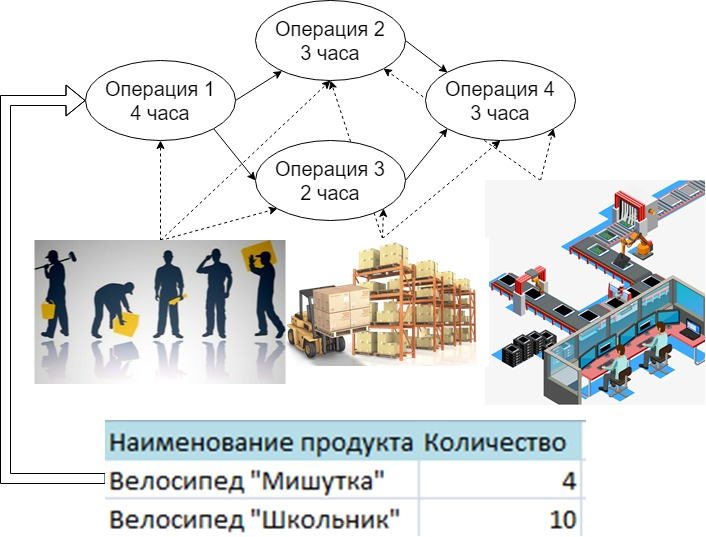
\includegraphics[width=1\linewidth]{fig/Prod1.jpg}}
    \caption{Модель производства}
    \label{ris:Prod1}
\end{figure}


\section{Математическое моделирование производственных процессов}

Для формализации процесса планирования в работе используются системы неравенств. Пример системы неравенств представлена на рисунке \ref{ris:sys1}. Система неравенств состоит из двух частей: статическую и динамическую. Статическая по своей сути копирует последовательность операций, описываемых в технологической карте. Динамическая накладывает дополнительные ограничения на систему неравенств, которая складывается из ресурсных зависимостей. Ресурсными зависимостями являются связи между операциями и фондом предприятия[3].

\begin{figure}[H]
    \center{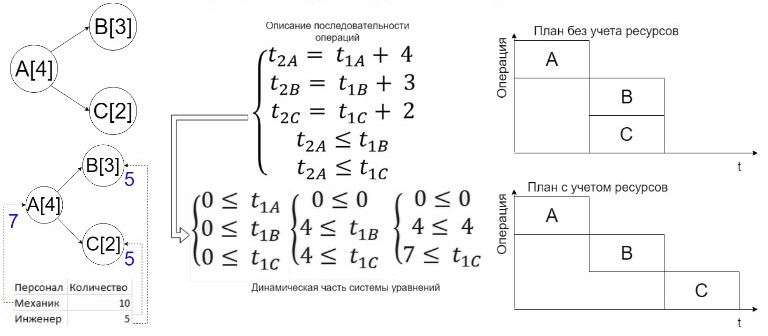
\includegraphics[width=1\linewidth]{fig/Screenshot_3.jpg}}
    \caption{Система неравенств}
    \label{ris:sys1}
\end{figure}

Таким образом планирование делится на шаги, каждый раз при этом формируются новые ограничения вводимые ресурсами[4].

\section{Предобработка технологических карт}

\section{Создание шаблона плана}

\section{Имитационное планирование}

Алгоритм планирования состоит из следующих этапов:
\begin{enumerate}
    \item Создание шаблона продуктов на основе заказа. Другими словами воспроизведение порядка операций указанной в технологической карте, статическая система неравенств.
    \item Создание плана на основе заказа. На данном этапе алгоритм создает шаблоны всех продуктов, которые перечислены в заказе, также учитывая количество одноименной продукции.
    \item Пошаговая реализация плана с учетом ресурсных ограничений. Добавление дополнительных ограничений в систему неравенств, которые динамически меняются с каждым шагом планирования.
\end{enumerate}
Работа имитационного моделирования представлена на рисунке \ref{ris:alg}
\begin{figure}[H]
    \center{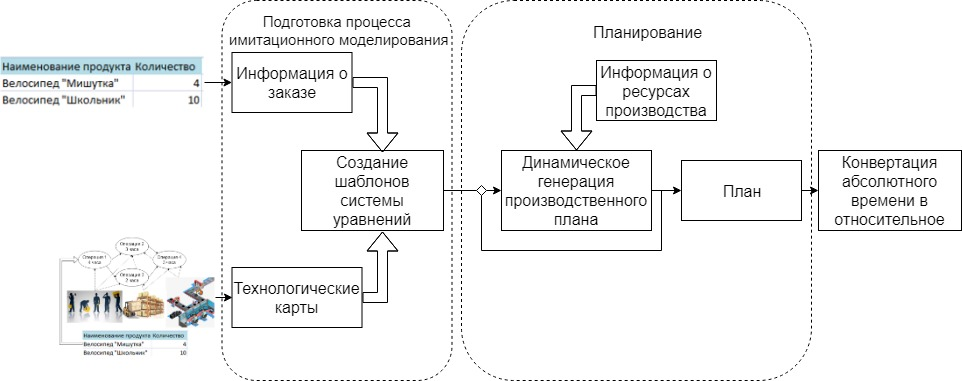
\includegraphics[width=1\linewidth]{fig/alg.jpg}}
    \caption{Визаулизация работы имитацонного моделирования}
    \label{ris:alg}
\end{figure}

\section{Оптимизация средствами имитацонного моделирования}

\subsubsection{Метод грубой силы}
Примером оптимизации может служить случайный выбор следующей операции при планировании, данный выбор возможен только в случаях одновременного выполнения нескольких независимых операций. Таким образом достигается вариативность при котором из разных реализаций, выбирается наилучший вариант. На рисунке (\ref{ris:Force}) изображены технологическая карта продукта и два плана, который были построены в результате случайного выбора операций. Как видно из рисунка (\ref{ris:Force}) первый план является более оптимальным по времени и ресурсам, чем второй.

\begin{figure}[H]
    \center{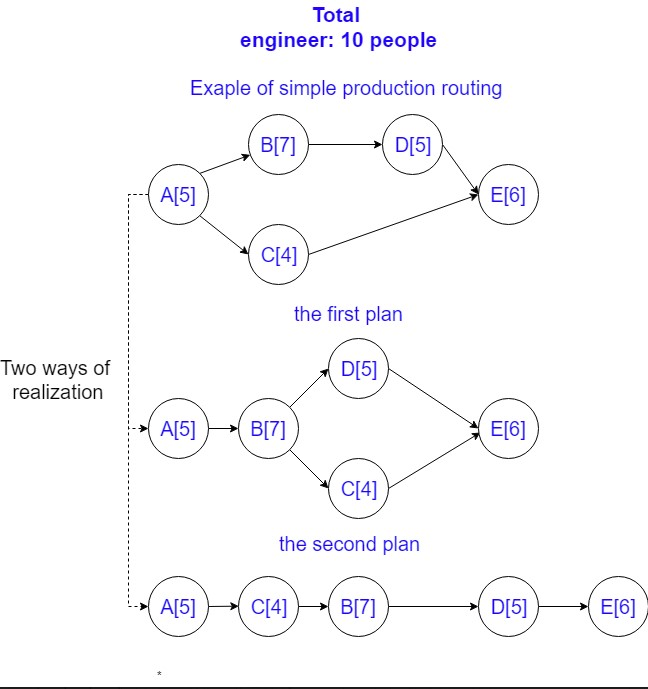
\includegraphics[width=1\linewidth]{fig/Force.jpg}}
    \caption{Два плана, полученные путем перебора исходной технологической карты}
    \label{ris:Force}
\end{figure}

\section{Результаты работы имитационной модели}